En este capítulo se mostrará el enfoque metodológico usado. Así como los riesgos, los recursos disponibles y los diagramas Gantt usados para la planificación de actividades y proyecto finalizado.

\newpage

\section{Investigación previa}
Debido a que a la gran mayoría de las necesidades actuales de cualquier aplicación que ofrezca un servicio necesita un servicio en la nube para almacenar datos, y con el estudio previo de la única implementación con éxito de un Sistema de SmartRural, decidimos escoger tecnologías híbridas que nos permitieran un desarrollo rápido, de caracter multiplataforma y escalable con el tiempo.

Así pues, para nuestro proyecto, escogimos el SDK Ionic, ya que, tiene una gran integración con la metología ágil y la PaaS de Azure Cloud.

\section{Enfoque metodológico}
Para el desarrollo de nuestro proyecto, hemos escogido la metodología ágil, por su gran versátilidad y la obligación al mismo tiempo de establecer ciclos iterativos donde se puedan sacar hitos del producto y así llegar mejor al producto final deseado.

Por ende, dentro de la metodología ágil, usaremos el más ampliamente usado, es decir, Scrum \cite{scrum}.

Por último, y para garantizar el éxito del proyecto, se han realizado revisiones periodicas por nuestra parte del producto en cada iteración, tanto de su dirección como de su calidad funcional y de implementación (Clean Code \cite{cleancode}\cite{cleancodebook}).

\section{Planificación del proyecto}
En este apartado, mostraremos el procedimiento de desarrollo de los componentes en 4 fases dentro de cada hito. Estas son:

\begin{itemize}
    \item Análisis: en esta fase vamos a definir los requisitos funcionales y no funcionales que forma el sistema dentro del hito. Después, los añadiremos a un Backlog para su posterior desarrollo.
    \item Diseño: en esta fase diseñaremos los prototipos de nuestro sistema y sus correspondientes diagramas conceptuales.
    \item Implementación: en esta fase implementaremos las tareas provenientes en el Backlog. Queda aclarar que muchas de las funcionalidades descritas en el Backlog tiene parte de implementación en el Backend y otra parte en el Frontend, así ha sido necesario el desarrollo de ambas partes al unisono para conseguir el funcionamiento deseado.
    \item Pruebas: por último, en esta fase se han desarrollado pruebas unitarias tanto en el Backend como en el Frontend. Se han omitido pruebas de integración, de aceptación, ...etc por qué con el software actual, no se han considerado necesarias.
\end{itemize}

\section{Diagrama Gantt}
En esta sección, mostraremos el diagrama de Gantt final de la ejecución del proyecto, que incluirá estimaciones iniciales más retrasos propios de no haber hecho en su momento bien las estimaciones o por circunstancias especiales. A continuación, en la Figura 3.1, se muestra el diagrama de Gantt.

\begin{figure}[H]
    \centering
    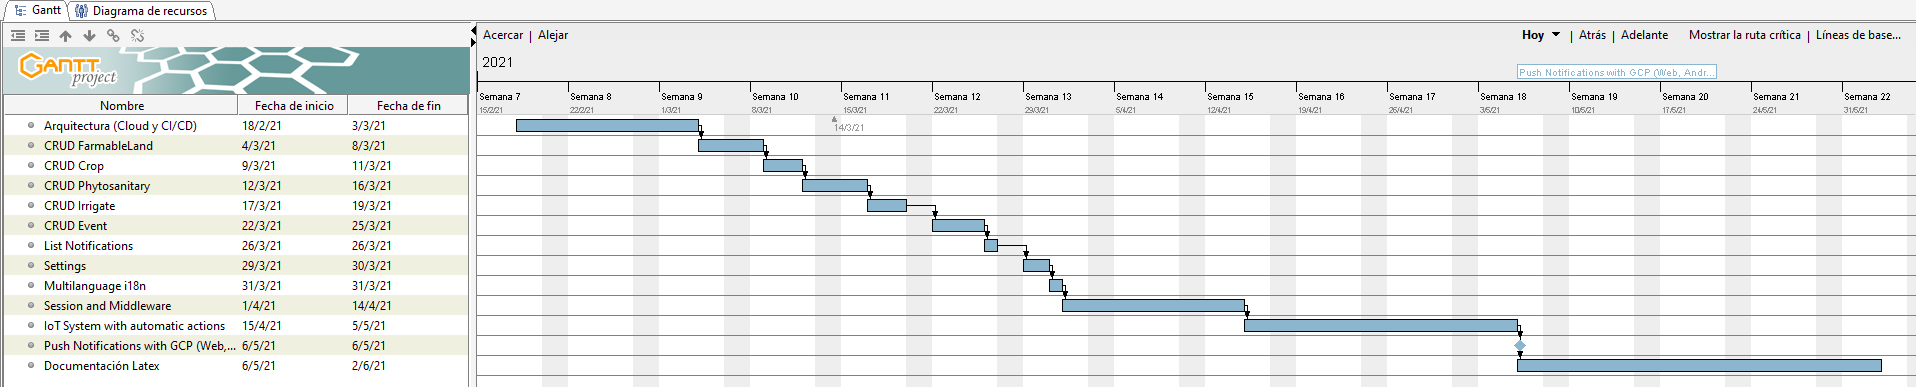
\includegraphics[width=1\linewidth,angle=90]{images/state-art/gantt.png}
    \caption{Estimaciones + Tiempo real de ejecución}
\end{figure}